\chapter[Lecture 11]{}\label{lec11}

32 point groups fall in two general categories
\begin{itemize}
\itemsep=0pt
\item[(i)] simple rotation group and
\item[(ii)] groups of higher symmetry
\end{itemize}

\section*{Simple rotation group}
One axis of highest symmetry. 
\begin{description}
\item[$C_{nv}$~:] Group contains a $\sigma_{v}$ reflection plane in addition to $C_{n}$. $\Rightarrow n$ reflection plane separated by $\frac{\pi}{n}$ around the rotation axis., $C_{n}$, $\sigma_{v}$.

\item[$C_{nh}$~:] $C_{n}+\sigma_{n}|C_{n},\sigma_{h}$

\item[$S_{n}$~:] $n$-fold improper rotation.

If $n$ is odd, it is similar to $C_{nh}$ 

$n$ is even $\to$ distinct group, which includes $C_{n/2}$ as a subgroup.

$S_{2}\equiv i$l $S_{4}$; $S_{6}\Rightarrow C_{3}\times i$ direct product group.

\item[$D_{n}$~:] $n$ $2$-fold axes perpendicular to $n$-fold axis.

$D_{2} \to$ Three mutually perpendicular $2$-fold axes. This group is sometimes called `$V$' group $\to$ Vierergruppe.

\item[$D_{nd}$~:] $D_{n}+\sigma_{d}$ reflection planes bisecting the angles between two-fold axes perpendicular to $C_{n}$ axis.

\item[$D_{nh}$~:] $D_{n}+\sigma_{n}$ (horizontal) reflection planes.

$D_{nh}$ has twice as many elements as $D_{n}$.
\end{description}
Some of the above can be expressed as direct product of simpler groups.
\begin{xalignat*}{2}
C_{2h} &= C_{2}\times i && D_{2h}=D_{2}\times i\\
C_{4h} &= C_{4}\times i && D_{4h}=D_{4}\times i\\
C_{6h} &= C_{6}\times i && D_{6h}=D_{6}\times i\\
S_{6} &= C_{3}\times i && D_{3d}=D_{3}\times i
\end{xalignat*}

\noindent
{\bf Group of higher symmetry :} There is no unique axis of highest symmetry.

Remaining $5$ point groups $T$, $T_{d}$, $T_{h}$, $0$, $0_{h}$ are the point groups of higher symmetry.
\begin{description}
\item[$T$ :] Comes from regular tetrahedron : smallest of the groups of higher symmetry. Contains 12 proper rotations, which take a regular tetrahedron into itself.
\begin{center}
\begin{minipage}[c]{6.2cm}
\begin{figure}[H]
\centering
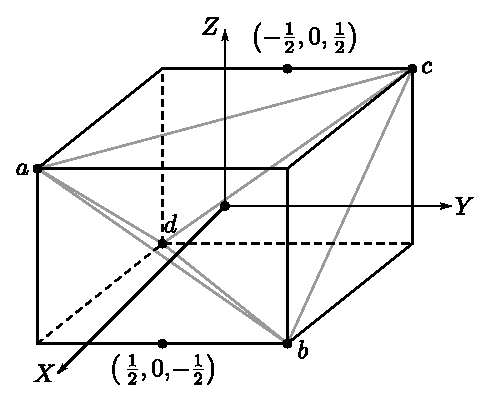
\includegraphics[scale=.8]{images/lecture11/fig1.eps}
\end{figure}
\end{minipage}
\qquad
\begin{minipage}[c]{6.2cm}
\begin{figure}[H]
\centering
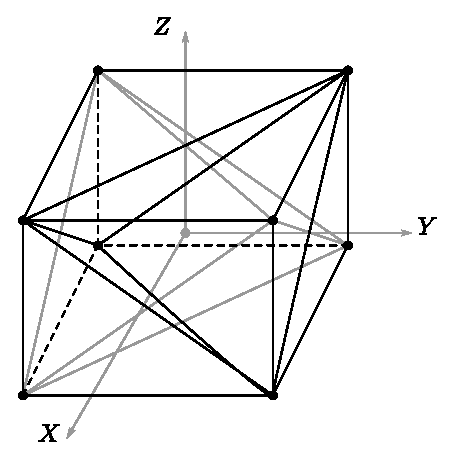
\includegraphics[scale=.8]{images/lecture11/fig2.eps}
\end{figure}
\end{minipage}
\end{center}
$abcd$ is the tetrahedron and $XYZ$ are normal to cube faces.

Covering operations : $E$; $3C_{2}$'s about $X$, $Y$ and $Z$; $8C_{3}$'s about body diagonals.

$E$, $3C_{2}$, $4C_{3}$, $4C'_{3}$, $8C_{3}$'s form two distinct classes for clock\-wise and anti-clock\-wise rotations because they are directed $\to$ there is no operation such as a perpendicular two-fold rotation will reverse the axis of rotation.

\item[$T_{d}$ :] Tetrahedral group : All elements in $T$ + reflections.

24 elements : 12 elements of $T$

+ 6 diagonal reflection plane normal to cube face $(\sigma_{d})$

+ 6 $S_{4}$ (positive and negative) $X$, $Y$ and $Z$ directions since reflection, $\sigma_{d}$ allows to interchange clockwise and anticlockwise rotations, all $8C_{3}$'s form one class in $T_{d}$. 

\item[$T_{h}$ :] Consists of 24 elements. $T_{h}=T\times i$ direct product.

A regular tetrahedron does not have $T_{h}$ symmetry as it does not have inversion symmetry.

\item[$O$ :] Octahedral group : 24 elements.

$E$, $8C_{3}$ about body diagonal

$3C_{2}$ about $X, Y, Z$ axes.

$6C_{4}$ about $X, Y, Z$ axes.

$6C_{2}$ about axis through origin parallel to face diagonals.
\end{description}

\noindent
{\bf Trigonal Prism?}
\begin{figure}[H]
\centering
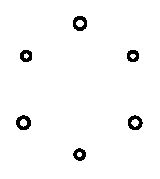
\includegraphics[scale=.8]{images/lecture11/fig2a.eps}
\end{figure}

Edge centres across a diagonal of a cube.

Consider body centre of a cube as origin, all face centres are occupied.
\begin{figure}[H]
\centering
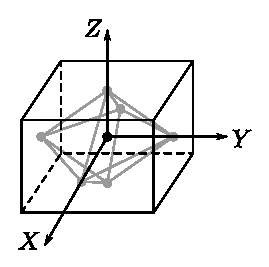
\includegraphics[scale=.8]{images/lecture11/fig3.eps}
\end{figure}

All $C_{3}$'s are equivalent as one can rotate the direction of diagonals by a $C_{2}$ existing in the group.

Two types of $C_{2}$'s form two different classes as axis of one can be used to generate axis of the other.
\begin{description}
\item[$O_{h}$ :] Full octahedral group $O_{h}=O\times i$
\begin{itemize}
\item Contains 48 elements and is the largest of all.

\item Includes improper rotations and reflections.

\item Each general point can be mapped into 48 distinct equivalent points.
\end{itemize}
\end{description}

\section*{One can include two other groups}
\begin{description}
\item[$C_{\infty v}$ :] $C_{\infty v}$ is the group of a general linear molecule, contains full rotational symmetry about the molecular axis and vertical reflection planes containing the molecular axis.

\item[$D_{\infty h}$ :] $D_{\infty h}$ : Contains a horizontal reflection plane and two fold symmetry about any axis on this plane passing through molecule centre.

$\to$ in addition to `$f$' it has $\sigma_{h}$ example $CO_{2}$; $ABA$ type molecule.
\end{description}

\noindent
{\bf Space Group :} {\em Semi-Direct} product group of Bravais Lattice translation $T_{R}$ and point group, $G\Rightarrow \fbox{$T_{R}\times G$}$.

32 point groups and 14 Bravais Lattices form 61 space groups [set red marks in the table] 7 additional orientations possible.

An object in with trigonal symmetry placed in Hexagonal lattice gives 5 more space groups.

Total $=61+5+7=73$.
\begin{landscape}
{\small
\renewcommand{\arraystretch}{1.05}
\begin{longtable}{l|l|l|c|l}
\captionsetup{justification=centering}
\caption{\em Classification of the point groups according to crystal systems}\\
\hline
\multicolumn{1}{c|}{{\bf\em System}} & \multicolumn{1}{c|}{{\it\bfseries Unit cell}/} & \multicolumn{1}{c|}{{\it\bfseries Groups}} & \multicolumn{1}{c|}{{\it\bfseries Number of}} & \multicolumn{1}{c}{{\color{red}{\it\bfseries No. of}}}\\
\multicolumn{1}{c|}{{\color{red}{\it\bfseries additional orientations}}} & \multicolumn{1}{c|}{{\color{red}{\it\bfseries Bravais Lattice}}} & & \multicolumn{1}{c|}{{\it\bfseries symmetry elements}} & \multicolumn{1}{c}{{\color{red}{\it\bfseries same group}}}\\
\hline
\endfirsthead
\hline
\multicolumn{1}{c|}{{\bf\em System}} & \multicolumn{1}{c|}{{\it\bfseries Unit cell}/} & \multicolumn{1}{c|}{{\it\bfseries Groups}} & \multicolumn{1}{c|}{{\it\bfseries Number of}} & \multicolumn{1}{c}{{\color{red}{\it\bfseries No. of}}}\\
\multicolumn{1}{c|}{{\color{red}{\it\bfseries additional orientations}}} & \multicolumn{1}{c|}{{\color{red}{\it\bfseries Bravais Lattice}}} & & \multicolumn{1}{c|}{{\it\bfseries symmetry elements}} & \multicolumn{1}{c}{{\color{red}{\it\bfseries same group}}}\\
\hline
\endhead
\hline
\endfoot
\endlastfoot
Triclinic & $a\neq b\neq c$\qquad \color{red}{1} & $C_{1}$ & 1 & \color{red}{$2\times 1=2$}\\
          & $\alpha\neq \beta\neq \gamma$ & $S_{2}(C_{i})$ & 2 & \\
\hline
Monoclinic & $a\neq b\neq c$ & $C_{1h}$ & 2 & \color{red}{$3\times 2=6$}\\
           & $\alpha=\gamma=\pi/2\neq\beta$\qquad \color{red}{2} & $C_{2}$ & 2 & \\
           & & $C_{2h}$ & 4 & \\
\hline
Orthorhombic & $a\neq b\neq c$ & $C_{2v}$ & 4 & \color{red}{$3\times 4=12$}\\
\color{red}{1 different orientation} & $\alpha=\beta=\gamma=\pi/2$\qquad \color{red}{4} & $D_{2}(V)$ & 4 & \\
                                     && $D_{2h}(V_{h})$ & 8 & \\
\hline
Tetragonal & $a=b\neq c$ & $C_{4}$ & 4 & \color{red}{$7\times 2=14$}\\
\color{red}{2 different orientations} & $\alpha=\beta=\gamma=\pi/2$\qquad \color{red}{2} & $S_{4}$ & 4 & \\
                                 & & $C_{4h}$ & 8 & \\
                                 & & $D_{2d}(V_{d})$ & 8 & \\
                                 & & $C_{4v}$ & 8 & \\
                                 & & $D_{4}$ & 8 & \\
                                 & & $D_{4h}$ & 16 & \\
\hline
Rhombohedral & $a=b=c$ & $C_{3}$ & 3 & \color{red}{$5\times 1=5$}\\
(trigonal) & $\alpha=\beta=\gamma<2\pi/3\neq \pi/2$ & $S_{6}(C_{3i})$ & 6 & \\
           & \multirow{3}{5cm}{5 more space group possible for having trigonal units arranged in Hexagonal lattice.\qquad {\color{red}{1}}} & $C_{3v}$ & 6 &\\
            & & $D_{3}$ & 6 &\\
            & & $D_{3d}$ & 12 &\\
\hline
Hexagonal & $a=b\neq c$ & $C_{3h}$ & 6 & {\color{red}{$7\times 1 = 7$}}\\
\color{red}{4 different orientations} & $\alpha=\beta=\pi/2$, $\gamma=2\pi/3$\qquad {\color{red}{1}} & $C_{6}$ & 6\\
 & & $C_{6h}$ & 12 & \\
 & & $D_{3h}$ & 12 & \\
 & & $C_{6h}$ & 12 & \\
 & & $D_{6}$ & 12 & \\
 & & $D_{6h}$ & 24 & \\
\hline
Cubic & $a=b=c$ & $T$ & 12 & {\color{red}{$5\times 3=15$}}\\
      & $\alpha=\beta=\gamma=\pi/2$\qquad {\color{red}{3}} & $T_{h}$ & 24 & \\
&& $T_{d}$ & 24 & \\
&& $O$ & 24 & \\
&& $O_{h}$ & 48 & \\
\hline
\multicolumn{3}{l}{\color{red}{7 additional orientation}} & {\color{red}{Total}} & {\color{red}{61}} \\
\hline
\end{longtable}}\relax
\end{landscape}

The assignments can be checked by using projection operator $P$.

\noindent
{\bf Symmorphic space group:} Each Bravais lattice points are oriented in the same way.

$\therefore$ \ There are 73 symmorphic space groups.

Remaining 157 space groups are {\bf non-symmorphic:} 

This contains additional operation, which cannot be simply compounded out of Bravais lattice translation and point group operation.

Among 157 space groups, 54 are half-symmorphic.

Due to other considerations, effective lattice constant becomes double.

\noindent
{\bf Notations:} Capital letter for Bravais lattice translation followed by symbols representing point group operations.
\begin{quote}
$P =$ Simple\qquad $A,B,C$ for base-centered

$I=$ Body-centered\qquad $F=$ Face centered
\end{quote}
For non-symmorphic space groups, symbols are complex for notations for point group operations and depends on crystal systems.
